\subsection{研究報告(姜)}
モノのインターネット(IoT)、ビッグデータ、人工知能技術の急速な発展に伴い、スマートシティは新しい研究分野として政府や産業界から非常に重視されている。様々なマルチモーダルの人の流れ移動データと都市のビッグデータ(スマートフォン位置データ、携帯電話の通話記録データ、GPS 軌跡データ、都市交通網データ、自然災害データ、伝染病データ、公共健康データなど)を統合、処理、分析し、新世代の人工知能技術(深層学習、強化学習、アンサンブル学習など)と結び付け、都市規模の人の流れの移動についてのモデリング、シミュレーション、予測を実現することにより、都市の交通整理、都市における緊急事態管理、災害時の人道支援、伝染病の拡大予防対策、公共の健康促進などの実現を目指す。これを背景にし、2019年度および2020年度に、引き続き私はデータ駆動型知能とアーバンコンピューティングについて研究活動を行ってきた。以下2点の研究プロジェクトをピックアップして詳しく紹介する。

\begin{itemize}
    \item 深層学習による都市レベルの群衆密度・流れの予測
    \item モビリティデータと医療データを統合したインフルエンザ流行の解析・予測
\end{itemize}

\subsubsection{深層学習による都市レベルの群衆密度・流れの予測}
大規模な都市区域を数々のきめ細かいメッシュグリッドへとメッシングすることで、連続的な期間における都市全体の群集や交通情報を映像のように表現し、各タイムスタンプを一枚の映像フレームとして扱うことができる。この考え方に基づき、都市全体の群集や交通に関する映像型の予測に対応するため一連の手法が提案された。現在、この手法群の評価は (1) 一部のモデルは他のモデルと比較できない、(2) 一部のモデルは群集流動データではなくタクシーや自転車などの交通流量のみによって検証されている、(3) 一部のモデルは天候データやPOIデータなどの外部データ源を活用している、(4) 一部のモデルは独自に設計したオブジェクト関数を用いている、(5) ホットステーションや朝の混雑時間における住宅地域といった一部の具体的な地域や時間帯によるケーススタディが欠けている、といった観点から未だに不十分である。本研究を通じ、我々は実世界のスマートフォンによるアプリケーションを通じて生成した集合的な人の移動に関する新たなデータセットを公開し、複数のオープンデータセットに基づいてそのような種類のアーバンコンピューティング問題に対する標準的なベンチマークを構築することを試みる。具体的には、(1) 群集および交通の密度予測、流出入予測といった2種類の古典的な問題を対象として設定する。前者では次のタイムスタンプにおいて各メッシュグリッドに何人または何台いるかを予測し、後者では次の時間間隔において各メッシュグリッドに何人または何台が流入または流出するかを予測する。過去に観察した複数ステップ分のデータを入力として扱い、次のステップにおける予測結果を出力として報告する。(2) 広く普及しているスマートフォンのアプリによるGPSログデータを用いて実世界の群集密度や流動を反映する新規データセットを作成する。次に、作成した新規データセットと既存のデータセットを用いて群集および交通の予測を実施できる。(3) 統一した目的関数であるMSEをモデルの訓練に採用し、外部データ源や関連する処理モジュールをモデルから除外する。それにより、時空間データの映像型モデリングに関する純粋な能力を公平に検証することができる。(4) 選択した地域の時系列の予測結果をケーススタディとして追加し、異なる場所や時間に対する有効性を実証する。

\subsubsection{モビリティデータと医療データを統合したインフルエンザ流行の解析・予測}
インフルエンザの流行により、健康被害や社会経済への影響が大きいため、インフルエンザがいつどこで発生し、感染がどのように拡大するかは重要な課題として政府や自治体に強調された。ビッグデータ時代、特にIoT(Internet of Things)時代に、従来の医学・免疫学分野になかったデータ駆動の方法を利用し、インフルエンザ流行のメカニズムを解明する。さらにそのメカニズムに基づいて流行状況の高精度な予測モデルを構築する。具体的に、本研究はブログウォッチャーGPS軌跡データ(人の移動モビリティデータとNDBレセプトデータ(医療データ)を利用する。ブログウォッチャーGPS軌跡データとは、提携アプリをダウンロードし、位置情報の取得を許可したユーザーのスマートフォン端末から、GPSで補足した経度緯度の位置情報である。一方、NDBレセプトデータとは、情報データベース(NDB)に蓄積されたレセプト情報・薬の処方情報などであり、インフルエンザ感染数のproxyとなるデータでもある。この二つのデータを組み合わせて、過去十年間の感染の広がり方の差異と人的空間移動の状況を解析し、まず地域間の人の移動がインフルエンザ感染・流行に寄与しているかを検証する;そして、関連していることが確定されればその人の移動によるインフルエンザ流行のメカニズムに基づき、リアルタイムかつ高精度のインフルエンザ流行状況の予測モデルを構築する。なお、本研究について、1)データへのアクセス(個人情報などの課題);2)データの粒度の違い、仕様の違い;3)データ量の多さ;4)モデリング手法などのチャレンジを克服するために、GPS軌跡データとNDB医療データを同時に用意するだけでなく、それぞれのデータに高度な解析能力を持つ時空間データ専門家及び医療データ専門家の高度なコラボレーションも欠かせない。異分野のデータと異分野の専門知識を備えた上で、次世代の人工知能技術(深層学習、強化学習、アンサンブル学習など)に基づき、新型のデータ統合解析技術・AI予測モデルを開発する。
% \begin{figure}[h]
% 	\centering	
% 	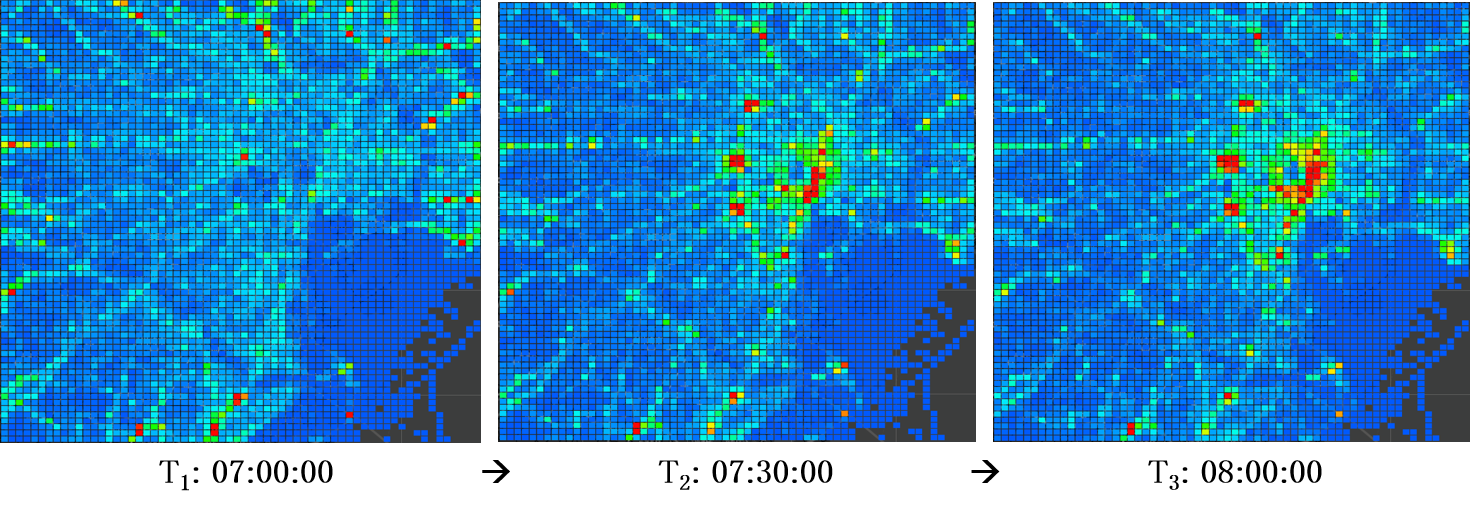
\includegraphics[width=7cm]{Kyo/figure/intro.png}
% 	\caption{都市全体の群集密度や流れは映像のように表現}
% 	\label{fig:intro}
% \end{figure}

% \begin{figure}[h]
%     \centering
%     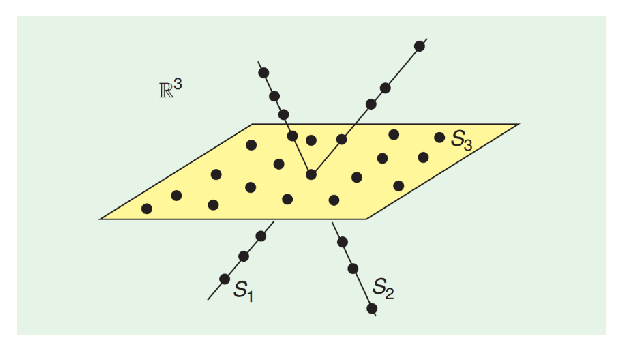
\includegraphics[width=7cm]{Matsushima/sc.eps}
%     \caption{部分空間クラスタリングの3次元の例(\cite{SC}から抜粋)。距離が近い点同士ではなく、同じ平面上もしくは同じ直線上(部分空間上)にある点同士をクラスタとみなす。}
%     \label{fig:my_label}
% \end{figure}